\section{Introduction}
\label{sec:intro}
Optical character recognition (OCR) engines always return a transcription, and modern end-to-end and
vision--language readers return fluent text even when they are wrong~\cite{fu2025ocrbenchv2,he2025seeing,gardella2026lowcer}.
Every consumer of OCR (key-information extraction from receipts and forms, archival search, accessibility, data entry)
must therefore decide, word by word, whether a transcription can be trusted or must be routed to a human. This is
\emph{OCR verification}: given a word image $x$ and a claim $h$ produced by an arbitrary, possibly black-box engine,
predict whether $h$ is exactly what is written in $x$. The three families of verifiers used in practice each have a
characteristic blind spot (Figure~\ref{fig:teaser}). \textbf{Engine confidence} is unavailable for many engines and
overconfident on fluent, plausible errors. \textbf{Re-recognition and voting} (accept $h$ iff a second recogniser
reads the same string~\cite{bautista2022parseq,li2023trocr,xiao2024florence}) is a binary test that inherits every
bias of the second recogniser. \textbf{Vision--language judges}~\cite{bai2025qwen25vl,zhang2025docrinspector} are
billions of parameters large, cannot be adapted from a handful of labels and, as we show, are poor at the
character-exact judgements verification needs.

\begin{figure}[t]
\centering
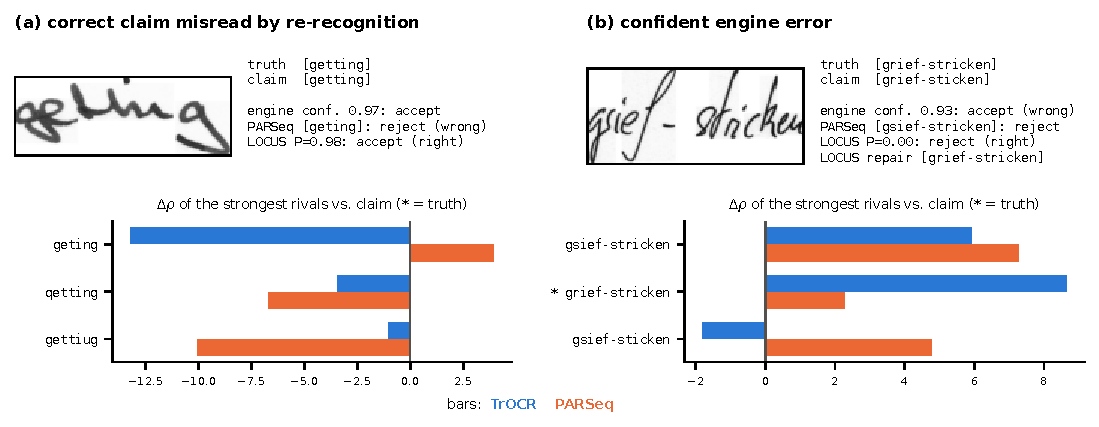
\includegraphics[width=0.85\linewidth]{figs/teaser.pdf}
\caption{\textbf{Why compare hypotheses instead of scoring one.} Two real IAM test words. (a) A correct claim that
PARSeq misreads, so re-recognition rejects it; PARSeq prefers its own reading (orange bar) but TrOCR strongly
disfavours it (blue bar), and \ours{}, which weighs both verifiers' evidence for every rival, accepts the claim (this
happens for 312 of the 419 correct IAM claims that PARSeq misreads). (b) A confident engine error that engine confidence
accepts; \ours{} rejects it and proposes the correct string. Bars: render-normalised evidence of the strongest rivals
relative to the claim ($*$: ground truth).}
\label{fig:teaser}
\end{figure}

\textbf{Key idea.} The right question is not ``does the image look like $h$?'' but ``is $h$ the best explanation
of the image among the strings it could have been confused with?'' An OCR error is a near miss: a confusable
substitution (\texttt{O}/\texttt{0}, \texttt{l}/\texttt{1}), a dropped or inserted glyph, or a case flip. We build
around every claim a small \emph{counterfactual string graph} of its OCR-plausible edits and test whether the claim is
a \emph{local optimum} of visual evidence on it. Two problems must be solved. First, the score must be \emph{visual}:
a recogniser's likelihood $s(v\mid x)$ mixes how well $v$ explains the pixels with how plausible $v$ is as a string,
so rare but correct strings are penalised. We cancel this prior with a \emph{render-normalised likelihood ratio}
$\rho(v)=s(v\mid x)-s(v\mid R(v))$, where $R(v)$ is a clean rendering of $v$. Second, the comparison must be learned
from very few labels: a relation-aware graph network with an explicit local-optimality readout is pretrained
\emph{without human labels} on images where two engines agree, paired with synthetic corruptions whose repair is known.

\textbf{Contributions.}
(1)~A formulation of OCR verification as testing the local optimality of a claim among OCR-plausible counterfactuals,
which also yields a repair proposal (Section~\ref{sec:method}).
(2)~Render-normalised evidence that removes the recogniser's string prior, computed with two frozen, architecturally
different recognisers.
(3)~\ours{}, a relation-aware GNN over counterfactual string graphs, pretrained label-free and adapted from
$k\in\{5,\dots,100\}$ labelled words per class.
(4)~A verification benchmark of \emph{real} OCR errors on five public datasets (forms, camera and scanned receipts,
handwriting, scene text) with two engines, and a comparison with engine and learned confidence, voting, three
re-recognition baselines and a 7B vision--language judge (Sections~\ref{sec:setup}--\ref{sec:results}).
(5)~An honest analysis: review cost, transfer, repair, document-level significance, recogniser dependence, rendering
sensitivity, message passing, and a manual audit with representative qualitative examples
(Sections~\ref{sec:analysis}--\ref{sec:qualitative}).
